\let\textcircled=\pgftextcircled
\chapter{FOUR}
..............
\section{Deep learning approaches}
In this section, we will show how we used deep learning to classify and diagnose plant leaf diseases. We focused on the use of convolution neural networks because they perform well when dealing with images.

During the experiments, we changed the hyperparameters and evaluated the results,We also demonstrate the utility of some pretrained models by fine-tuning them to fit our dataset.

Finally, comparisons for the various experiments are provided.
\section{Convolution neural networks}
\subsection{First CNN architecture From scratch}
the first CNN experiment architecture has  150 X 150 X 3 input shape with tomato dataset and 256 X 256 X 3 with plantVillage dataset, is composed of Convolution layer with 64 filters of size 3x3 followed by a max pooling layer with a window of size 2x2 , a second convolutional layer with the same configuration but only with 32 filters and a second max pooling layer exactly the same of the first. \\
A fully connected layer of 128 units and an output layer with 10 units (in case of tomato Dataset) and 38 units (in case of plantVillage dataset) according to the number of classes .
We will be using the Rectified linear unit (ReLU) activation
function for all the layers except the final output layer with a softmax function,
The training was done
during 100 epochs optimized by AdamOptimizer.\\
we train this model on two datasets described recently in \ref{Dataset description}
The hyperparameters of the architecture are
describe in two tables one with plantvillage dataset and another with tomato dataset.\\

\begin{table}[h]
\begin{tabular}{@{}|p{9cm}|p{3cm}|@{}}
\hline
 \centering \textbf{Parameter} & \textbf{Value}  \\ \hline
 Number of epochs & 100  \\  \hline
 Optimizer & Adam \\ \hline
 Dropout rate & / \\ \hline
 Number of learnable parameters & 5,319,978 \\ \hline
 One epoch training duration & 85s \\ \hline
 
\end{tabular}
\caption{hyperparameters of first cnn with Tomato dataset}
\end{table}

\begin{table}[h]
\begin{tabular}{@{}|p{9cm}|p{3cm}|@{}}
\hline
 \centering \textbf{Parameter} & \textbf{Value}  \\ \hline
 Number of epochs & 100  \\  \hline
 Optimizer & Adam \\ \hline
 Dropout rate & / \\ \hline
 Number of learnable parameters & 31,520,326 \\ \hline
 One epoch training duration & 132s \\ \hline
 
\end{tabular}
\caption{hyperparameters of first cnn with plantvillage dataset}
\end{table}
\begin{itemize}
    \item We obtained from this experiment an accuracy of 99.61\% in training set and 91.10\% in validation set with tomato dataset.
    \item with plantvillage dataset We obtained from this architecture an accuracy of 99.94\% in training set and only 58.48\% in validation set.
\end{itemize}
\begin{figure}[h]
    \centering
    \includegraphics[height=75mm]{chapters/chapter04/fig04/CNN1TD_Our_Proposed_Architecture_1_CNN_From_Scratch_Tomato_Dataset.png}
    \caption{First CNN architecture From scratch}
    \label{fig:my_label}
\end{figure}
%%%%%%%%%%%%%%%%%%%%%%%%%%%%%%%%%%%%%%%%%%%%%%%%%%%%%%%%%%%%
\subsection{Second CNN architecture From scratch}
the second CNN experiment architecture has 150 X 150 X 3 input shape with tomato dataset and 256 X 256 X 3 with plantVillage dataset ,is composed of Convolution layer with 32 filters of size 3x3 followed by a max pooling layer with a window of size 2x2 , a second convolutional layer with the same configuration and number of filters(32) and a second max pooling layer exactly the same of the first. \\
Two fully connected layers of 128 units and an output layer with 10 units(in case of tomato Dataset) and 38 units (in case of plantVillage dataset) according to the number of classes .
We will be using the Rectified linear unit (ReLU) activation
function for all the layers except the final output layer with a softmax function,
The training was done
during 100 epochs optimized by AdamOptimizer.\\
we train this model on two datasets described recently in \ref{Dataset description}
The hyperparameters of the architecture are
describe in two tables one with plantvillage dataset and another with tomato dataset.\\

\begin{table}[H]
\begin{tabular}{@{}|p{9cm}|p{3cm}|@{}}
\hline
 \centering \textbf{Parameter} & \textbf{Value}  \\ \hline
 Number of epochs & 100  \\  \hline
 Optimizer & Adam \\ \hline
 Dropout rate & / \\ \hline
 Number of learnable parameters & 5,336,490 \\ \hline
 One epoch training duration & 78s \\ \hline
 
\end{tabular}
\caption{hyperparameters of second cnn with Tomato dataset}
\end{table}

\begin{table}[H]
\begin{tabular}{@{}|p{9cm}|p{3cm}|@{}}
\hline
 \centering \textbf{Parameter} & \textbf{Value}  \\ \hline
 Number of epochs & 100  \\  \hline
 Optimizer & Adam \\ \hline
 Dropout rate & / \\ \hline
 Number of learnable parameters & 15,776,710 \\ \hline
 One epoch training duration & 60s \\ \hline
 
\end{tabular}
\caption{hyperparameters of second cnn with plantvillage dataset}
\end{table}
\begin{itemize}
    \item We obtained from this experiment an accuracy of 99.42\% in training set and 87.20\% in validation set with tomato dataset.
    \item with plantvillage dataset We obtained from this architecture an accuracy of 98.90\% in training set and only 57.20\% in validation set.
\end{itemize}
%%%%%%%%%%%%%%%%%%%%%%%%%%%%%%%%%%%%%%%%%%%%%%%%%%%%%%%%%%%%%
\subsection{Third CNN architecture From scratch}
the Third CNN experiment architecture has 150 X 150 X 3 input shape with tomato dataset and 256 X 256 X 3 with plantVillage dataset ,is composed of Convolution layer with 32 filters of size 3x3 followed by a batch normalization layer then
a max pooling layer with a window of size 2x2 , a second convolutional layer with the same configuration and number of filters(32) then a droupout with 20\%, another batch normalisation layer
and a second max pooling layer exactly the same of the first. 
a fully connected layers of 128 units and a dropout of 30\% finally an output layer with 10 units(in case of tomato Dataset) and 38 units (in case of plantVillage dataset) according to the number of classes .
We will be using the Rectified linear unit (ReLU) activation
function for all the layers except the final output layer with a softmax function,
The training was done
during 100 epochs with a batch size of 64 optimized by AdamOptimizer.\\
we train this model on two datasets described recently in \ref{Dataset description}
The hyperparameters of the architecture are
describe in two tables one with plantvillage dataset and another with tomato dataset.\\

\begin{table}[H]
\begin{tabular}{@{}|p{9cm}|p{3cm}|@{}}
\hline
 \centering \textbf{Parameter} & \textbf{Value}  \\ \hline
 Number of epochs & 100  \\  \hline
 batch size & 64 \\ \hline
 Optimizer & Adam \\ \hline
 Dropout rate & 0.3 and 0.2 \\ \hline
 Number of learnable parameters & 5,320,106 \\ \hline
 One epoch training duration & 90s \\ \hline
 
\end{tabular}
\caption{hyperparameters of third cnn with Tomato dataset}
\end{table}

\begin{table}[H]
\begin{tabular}{@{}|p{9cm}|p{3cm}|@{}}
\hline
 \centering \textbf{Parameter} & \textbf{Value}  \\ \hline
 Number of epochs & 100  \\  \hline
 Optimizer & Adam \\ \hline
 batch size & 64 \\ \hline
 Dropout rate & 0.3 and 0.2\\ \hline
 Number of learnable parameters & 15,760,326 \\ \hline
 One epoch training duration & 125s \\ \hline
 
\end{tabular}
\caption{hyperparameters of Third cnn with plantvillage dataset}
\end{table}
\begin{itemize}
    \item We obtained from this experiment an accuracy of 95.28\% in training set and 84.90\% in validation set with tomato dataset.
    \item with plantvillage dataset We obtained from this architecture an accuracy of 98.59\% in training set and only 86.33\% in validation set.
\end{itemize}

%%%%%%%%%%%%%%%%%%%%%%%%%%%%%%%%%%%%%%%%%%%%%%
\subsection{Fourth CNN architecture From scratch}
the Fourth CNN experiment architecture has 150 X 150 X 3 input shape with tomato dataset and 256 X 256 X 3 with plantVillage dataset ,is composed of Convolution layer with 32 filters of size 3x3 followed by a batch normalization layer then
a max pooling layer with a window of size 2x2 , a second convolutional layer with the same configuration and less number of filters(24) then a dropout with 20\% followed by a batch normalization and max pooling layer with a window of size 2 X 2,
a third convolutional layer with 24 filters of size 3 X 3
followed by a batch normalization and max pooling layer with a window of size 2 X 2
two fully connected layers of 128 units and finally an output layer with 10 units(in case of tomato Dataset) and 38 units (in case of plantVillage dataset) according to the number of classes .
We will be using the Rectified linear unit (ReLU) activation
function for all the layers except the final output layer with a softmax function,
The training was done
during 100 epochs optimized by AdamOptimizer.\\
we train this model on two datasets described recently in \ref{Dataset description}
The hyperparameters of the architecture are
describe in two tables one with plantvillage dataset and another with tomato dataset.\\

\begin{table}[H]
\begin{tabular}{@{}|p{9cm}|p{3cm}|@{}}
\hline
 \centering \textbf{Parameter} & \textbf{Value}  \\ \hline
 Number of epochs & 100  \\  \hline
 Optimizer & Adam \\ \hline
 Dropout rate & 0.2 \\ \hline
 One epoch training duration & 75s \\ \hline
 
\end{tabular}
\caption{hyperparameters of Fourth cnn with Tomato dataset}
\end{table}

\begin{table}[H]
\begin{tabular}{@{}|p{9cm}|p{3cm}|@{}}
\hline
 \centering \textbf{Parameter} & \textbf{Value}  \\ \hline
 Number of epochs & 100  \\  \hline
 Optimizer & Adam \\ \hline
 Dropout rate & 0.2\\ \hline
 One epoch training duration & 160s \\ \hline
 
\end{tabular}
\caption{hyperparameters of Fourth cnn with plantvillage dataset}
\end{table}
\begin{itemize}
    \item We obtained from this experiment an accuracy of 98.54\% in training set and 88.10\% in validation set with tomato dataset.
    \item with plantvillage dataset We obtained from this architecture an accuracy of 99.83\% in training set and only 88.48\% in validation set.
\end{itemize}
%%%%%%%%%%%%%%%%%%%%%%%%%%%%%%%%%%%%%%%%%%%%%%%%%%%%%%%%

\subsection{Last CNN architecture From scratch}
the Fifth CNN experiment architecture has introduced by some preprocessing layers : \textbf{Rescaling} values of our images by changing the interval from [0-255] to [0-1] we can also call it normalization ,\textbf{Random Flip},\textbf{Random rotation} and \textbf{Random zoom} this tasks will perform during the training
we put 256 X 256 X 3 as input shape, the first Convolution layer has 64 filters of size 3x3 followed by a max pooling layer with a window of size 2x2 , a second convolutional layer with the same configuration and more number of filters(128) then a dropout with 25\% followed by a max pooling layer with a window of size 2 X 2,
a third convolutional layer with 256 filters of size 3 X 3
followed by a  max pooling layer and a dropout with 25\%
two fully connected layers of 256 and 512 units and finally an output layer with 10 units(in case of tomato Dataset) and 38 units (in case of plantVillage dataset) according to the number of classes .
We will be using the Rectified linear unit (ReLU) activation
function for all the layers except the final output layer with a softmax function,
The training was done
during 100 epochs optimized by AdamOptimizer.\\
we train this model on two datasets described recently in \ref{Dataset description}
The hyperparameters of the architecture are
describe in two tables one with plantvillage dataset and another with tomato dataset.\\

\begin{table}[H]
\begin{tabular}{@{}|p{9cm}|p{3cm}|@{}}
\hline
 \centering \textbf{Parameter} & \textbf{Value}  \\ \hline
 Number of epochs & 100  \\  \hline
 batch size & 32 \\ \hline
 Optimizer & Adam \\ \hline
 Dropout rate & 0.25 \\ \hline
 One epoch training duration & 111s \\ \hline
 Number of learnable parameters & 13,942,922 \\ \hline
\end{tabular}
\caption{hyperparameters of last cnn with Tomato dataset}
\end{table}

\begin{table}[H]
\begin{tabular}{@{}|p{9cm}|p{3cm}|@{}}
\hline
 \centering \textbf{Parameter} & \textbf{Value}  \\ \hline
 Number of epochs & 100  \\  \hline
 batch size & 32 \\ \hline
 Optimizer & Adam \\ \hline
 Dropout rate & 0.25 \\ \hline
 One epoch training duration & 149s \\ \hline
 Number of learnable parameters & 26,792,614 \\ \hline
\end{tabular}
\caption{hyperparameters of Last cnn with plantvillage dataset}
\end{table}
\begin{itemize}
    \item We obtained from this experiment an accuracy of 98.99 \% in training set and 93.72\% in validation set with tomato dataset.
    \item with plantvillage dataset We obtained from this architecture an accuracy of 97.59\% in training set and only 93.95\% in validation set.
\end{itemize}
%%%%%%%%%%%%%%%%%%%%%%%%%%%%%%%%%%%%%%%%%%%%%%%%%%%%%%%%
\section{Pretrained models ( Transfer learning )}
Transfer learning is a popular method in computer vision because it allows us to build accurate models in a time saving way \cite{art39}. With transfer learning, instead of starting the learning process from scratch, you start from patterns that have been learned when solving a different problem. This way you leverage previous learnings and avoid starting from scratch \ref{Transfer learning} \\
\begin{figure}[H]
    \centering
    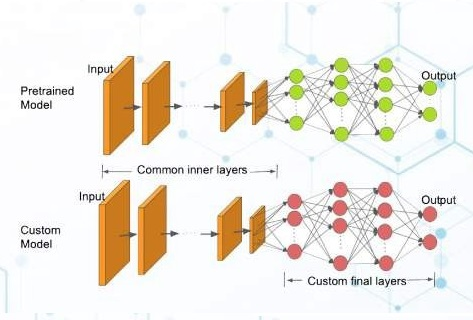
\includegraphics[width=1\textwidth]{chapters/chapter04/fig04/transfer.jpeg}
    \caption{Transfer learning process}
    \label{fig:my_label}
\end{figure}
in this section we will try some pretrained models to classify our images and see if
these models will give better results compared to our proposed architectures.we will divide this phase into x main approaches (VGG 16, Resnet , Mobile NET )
\subsection{Modified VGG-16 pretrained model}
We tuned VGG16 model by removing the top layer (instruction in keras : include-top=False) and unfrozen the model(instruction in keras trainable = true),
the input data of this model (tomato dataset) has a shape (128,128,3) and
(256,256,3) with plantVillage dataset it was normalized and augmented by a horizontal flip, rotation, zoom and rescaling values.\\
we added a batch normalization layer followed by two fully connected layers the first with 256 units and the second with 512 units then we added a dropout with 40\% , 
and changed the output
layer to have ten units (in case of tomato Dataset) and 38 units (in case of plantVillage
dataset) according to the number of classes . We will be using the Rectified linear unit (ReLU)
activation function for all the layers except the final output layer with a softmax function, using Early Stopping \ref{Early stopping} The
training was done during 29 epochs optimized by AdamOptimizer with learning rate equal to 0.001, 
It took \textbf{26 minutes} with tomato Dataset and 
\textbf{4 hours 20 minutes} with PlantVillage Dataset of training using google colab pro \ref{Google Colab Pro}, 
The hyperparameters of the architecture are
describe below.\\

\begin{table}[H]
\begin{tabular}{@{}|p{9cm}|p{3cm}|p{3cm}|@{}}
\hline
 \centering \textbf{Parameter} & \textbf{Tomato Dataset} & \textbf{PlantVillage Dataset} \\ \hline
 Number of epochs & 29  & 20 \\  \hline
 batch size & 30 & 30\\ \hline
 Optimizer & Adam & Adam\\ \hline
 Dropout rate & 0.4 & 0.4\\ \hline
 Learning rate & 0.001 & 0.001 \\ \hline
\end{tabular}
\caption{hyperparameters of Vgg16}
\end{table}
\begin{itemize}
    \item We obtained from this experiment an accuracy of 97.5\% on validation set and 97.8\% on test set with tomato dataset.
    \item We obtained from this experiment an accuracy of 99.13\% on validation set and 98.37\% on test set with PlantVillage dataset.
\end{itemize}
\begin{figure}[H]
    \centering
    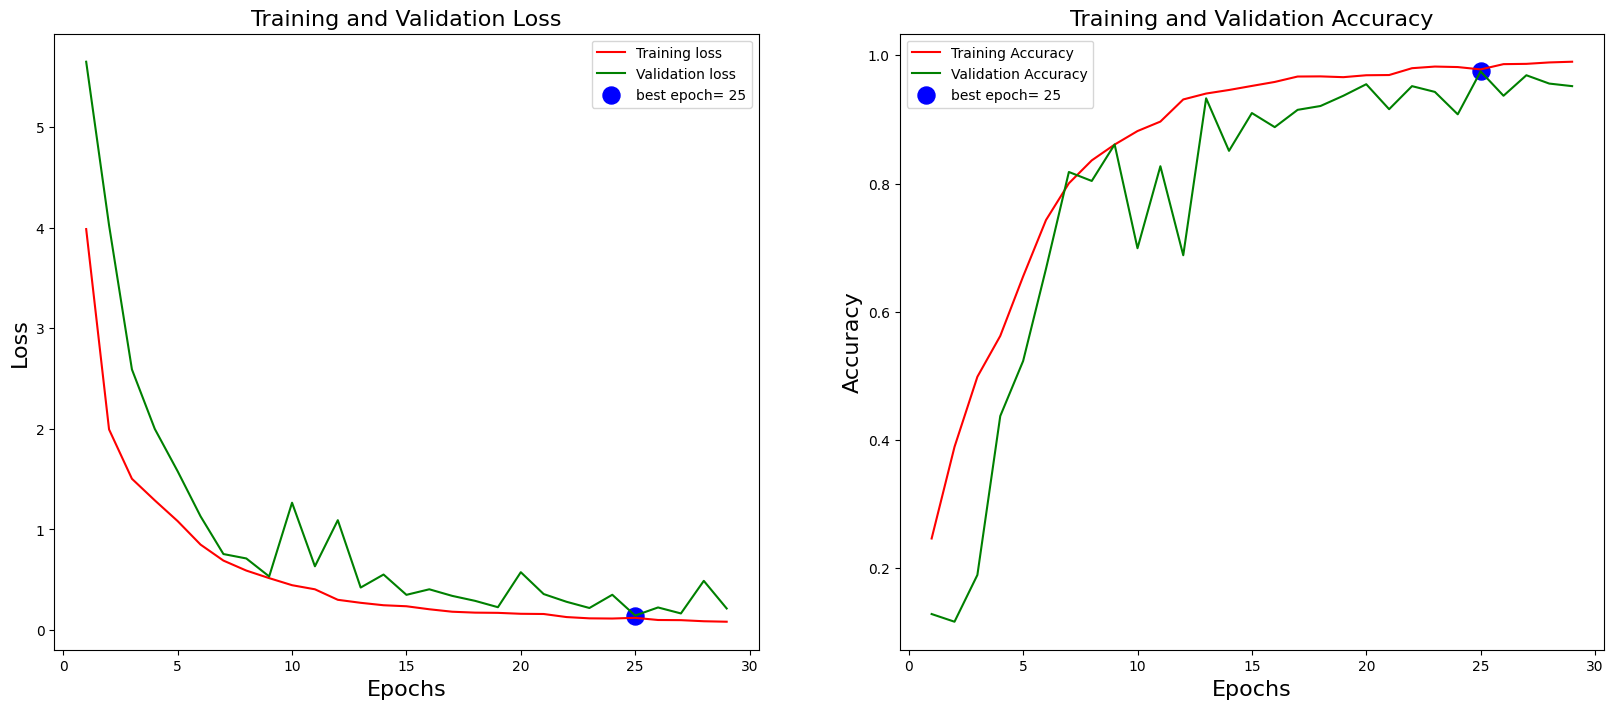
\includegraphics[width=1\textwidth]{chapters/chapter04/fig04/tomato ds_VGG16.png}
    \caption{Training and validation loss and accuracy Vgg16 Tomato Dataset}
\end{figure}
\begin{figure}[H]
    \centering
    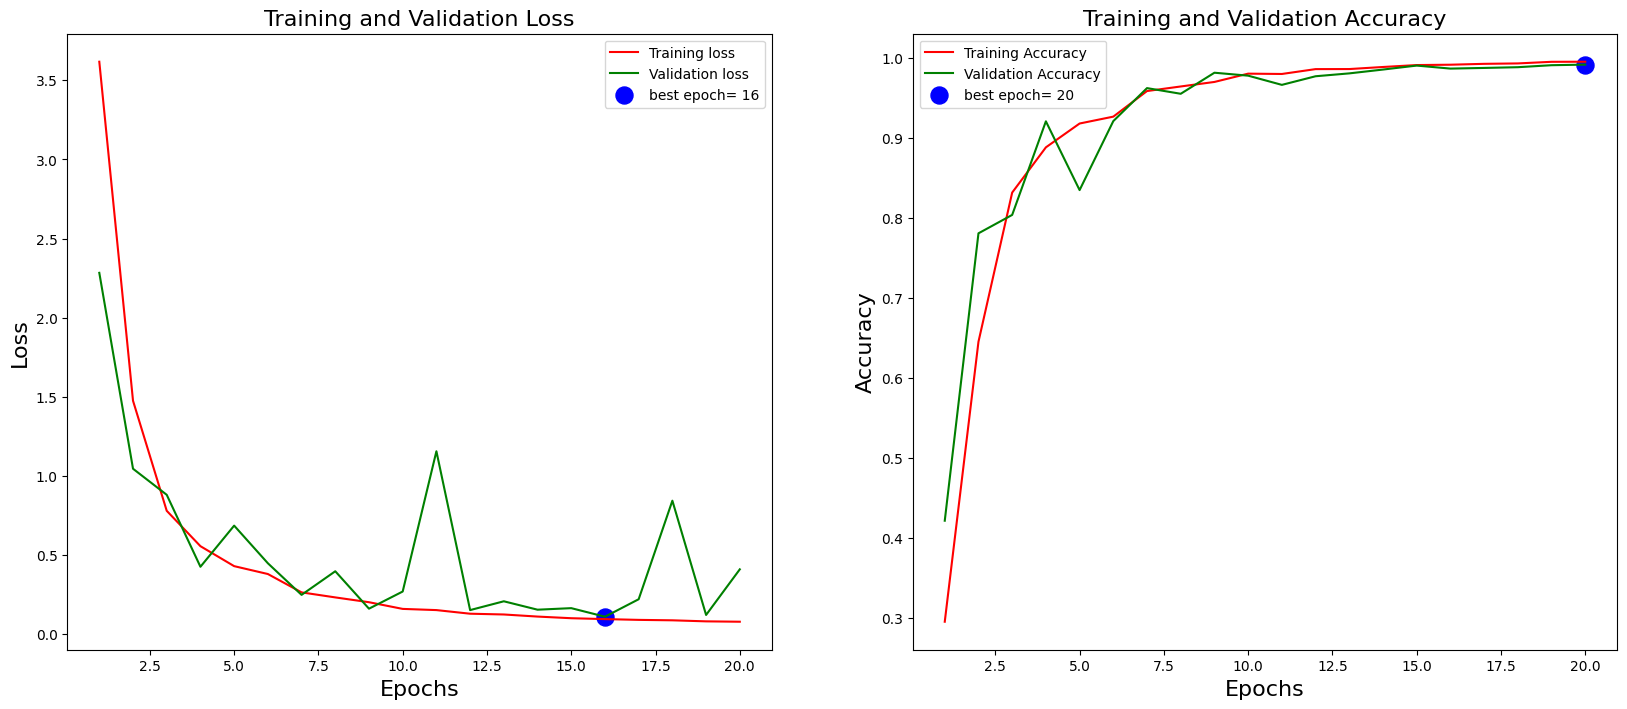
\includegraphics[width=1\textwidth]{chapters/chapter04/fig04/pv ds_VGG16.png}
    \caption{Training and validation loss and accuracy Vgg16 PlantVillage Dataset}
\end{figure}
\begin{figure}[H]
    \centering
    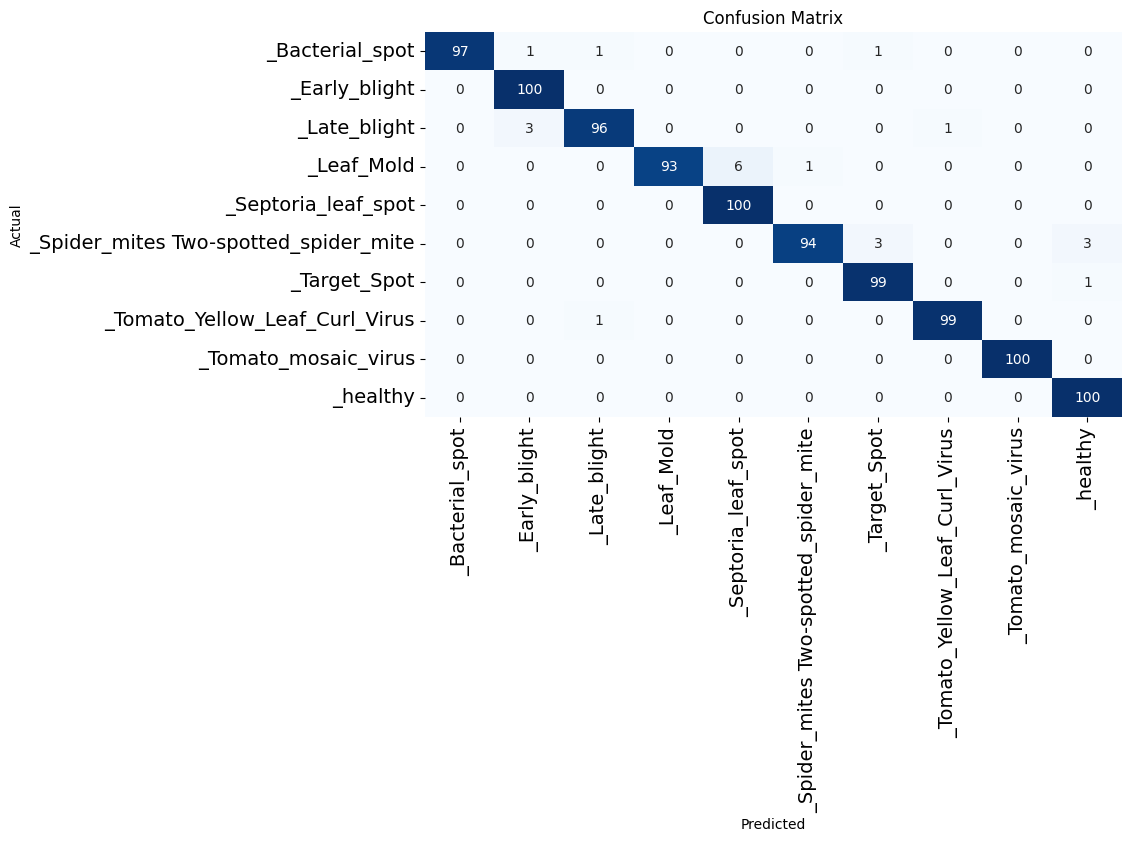
\includegraphics[width=1\textwidth]{chapters/chapter04/fig04/tomato ds_VGG16 cm.png}
    \caption{Confusion Matrix Vgg16 Tomato Dataset}
\end{figure}
\begin{figure}[H]
    \centering
    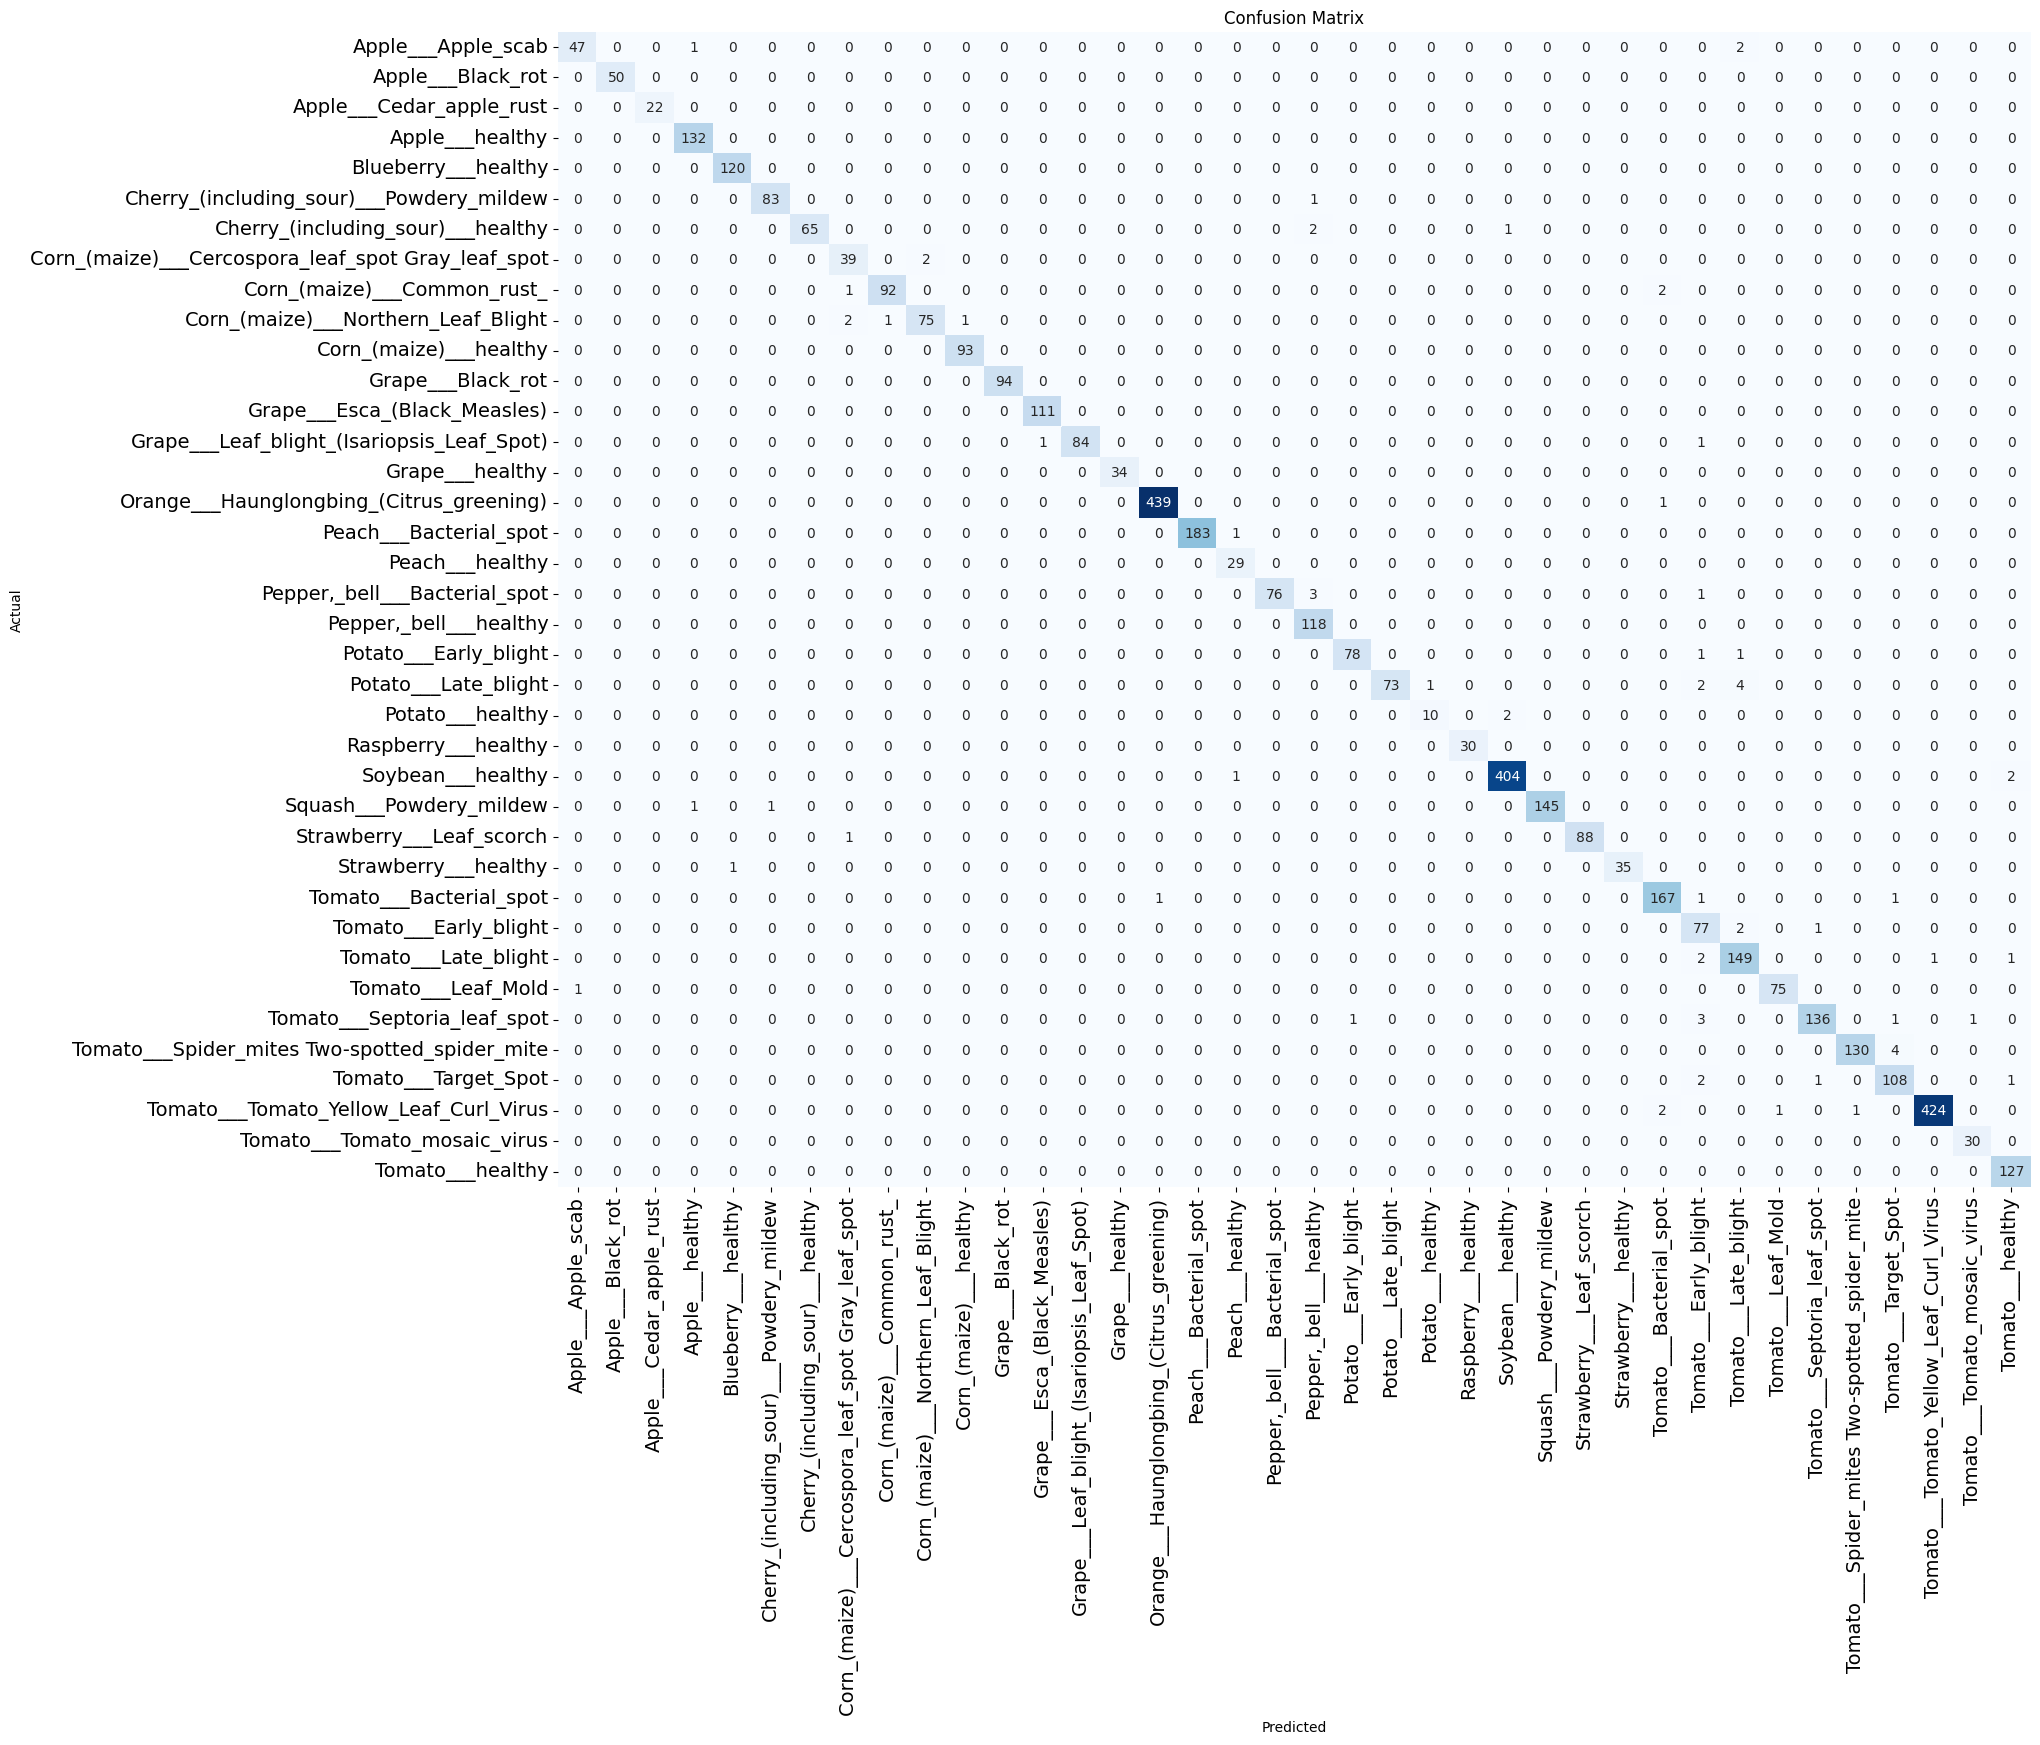
\includegraphics[width=1\textwidth]{chapters/chapter04/fig04/pv ds_VGG16 cm.png}
    \caption{Confusion Matrix Vgg16 PlantVillage Dataset}
\end{figure}
\subsection{VGG-19 pretrained model}
\subsection{AlexNet pretrained model}
\subsection{ResNet pretrained model}
ResNet \cite{art32}, proposed by Microsoft researchers is similar to VGG but deeper; it introduced a new concept
called residual learning that helps go very deeply. Residual learning allows training
efficiently very deep networks having up to a depth of 152 layers.\\

We tuned the ResNet model by removing the top layer (instruction in keras : include-top=False) and
frozen the model(instruction in keras trainable = False), and changed the output layer to have
ten neurons in case of tomato dataset or 38 neurons in case of PlantVillage dataset corresponding to number of classes . the input data of this model (tomato dataset) has a
shape (224,224,3) similar to imageNet and (256,256,3) with plantVillage dataset,
it was normalized and augmented by a horizontal flip and zoom and rescaling.\\

The training .... 
\subsection{Inception pretrained model}
\subsection{Xception pretrained model}
\subsection{Mobile Net Pretrained Model}














